\documentclass[xcolor=(list of options)]{beamer}
\usepackage[spanish]{babel}
\selectlanguage{spanish}
\usepackage[utf8]{inputenc}
\mode<presentation> {

%----------------Beamer Themes--------------------

\usetheme{Boadilla}

%--------------------Beamer Font & Colors----------

\usecolortheme{seahorse}

%-------------------Beamer Options --------------------

\setbeamertemplate{navigation symbols}{} % To add the navigation symbols from the bottom of all slides comment this line
}

%-------------------Package----------------------------
\RequirePackage{natbib}
\usepackage{graphicx} 
\usepackage{booktabs} % use of \toprule, \midrule and \bottomrule in tables
\usepackage{tikz}
\usepackage{pgfplots}
\usepackage{multirow}
\usepackage{multicol}
\usepackage{amsmath}
\usepackage{hhline}
\usepackage[export]{adjustbox} %para posicionar imagenes(ej, left, right)

%---Librerias de Tikz -----------------------------
\usetikzlibrary{arrows,calc}
\usetikzlibrary{intersections}
\usetikzlibrary{pgfplots.fillbetween}
\usetikzlibrary{patterns}
\usetikzlibrary{plotmarks}
\usetikzlibrary{calc}
\usetikzlibrary{matrix}
\usetikzlibrary{positioning}
\usepackage{relsize}
\usepackage[nointegrals]{wasysym}
\usepackage{caption}
\usepackage{bigints}
\usepackage{xcolor}
%---------------------------------------------------------------------------------

%-----------Tikz Layers---------------------------------
\pgfdeclarelayer{ft}
\pgfdeclarelayer{bg}
\pgfsetlayers{bg,main,ft}
%---------------------------------------------------------


%--------Definiciones de Operadores --------------
\DeclareMathOperator*{\argmax}{arg\,max}
\def\checkmarkt{\tikz\fill[scale=0.4](0,.35) -- (.25,0) -- (1,.7) -- (.25,.15) -- cycle;} 
\newcommand{\bigqm}[1][1]{\text{\larger[#1]{\textbf{?}}}}
\let\Tiny=\tiny % fix issue font name beamer
\makeatletter

\newcommand\mathcircled[1]{%
  \mathpalette\@mathcircled{#1}%
}
\newcommand\@mathcircled[2]{%
  \tikz[baseline=(math.base)] \node[draw,circle,inner sep=1pt] (math) {$\m@th#1#2$};%
}

%north west lines pattern density ajusted
\pgfdeclarepatternformonly[\LineSpace,\LineSpaceColor]{MNWL}{\pgfqpoint{-1pt}{-1pt}}{\pgfqpoint{\LineSpace}{\LineSpace}}{\pgfqpoint{\LineSpace}{\LineSpace}}%
{
    \pgfsetcolor{\tikz@pattern@color}
    \pgfsetlinewidth{0.4pt}
    \pgfpathmoveto{\pgfqpoint{0pt}{\LineSpace}}
    \pgfpathlineto{\pgfqpoint{\LineSpace + 0.1pt}{-0.1pt}}
    \pgfsetstrokecolor{\LineSpaceColor}%        % <-- added
    \pgfusepath{stroke}
}
\makeatother

\newdimen\LineSpace
\tikzset{
    line space/.code={\LineSpace=#1},
    line space=6pt, %this ajust density of MNWL
    line color/.store in=\LineSpaceColor,      % <-- added
    line color=black,
} %line set color in custom parttern check line 665-667 for an example

%----------------------------------------------------------------------------------------
%	           Slide Inicial
%----------------------------------------------------------------------------------------
 

\title[ECO -TS101]{Econometr\'\i{}a de Series de Tiempo} 
\subtitle{T\'opico V.- Non-linear Models: Volatility Forecasting}

%Profesores

\author{Marcelo Villena Ch., PhD} 

%-----------------------------------------------------------------

\institute[UAI] % Your institution as it will appear on the bottom of every slide, may be shorthand to save space
{
Universidad Adolfo Ib\'a\~nez 
 \\ % institution for the title page
\medskip
}
\date{} % Date, can be changed to a custom date

%-------------------Figure Settings-------------------
\pgfplotsset{ % Here we specify options for all figures in the document
  compat=1.8, % Which version of pgfplots do we want to use?
  legend style = {font=\small\sffamily}, % Legends in a sans-serif font
  label style = {font=\small\sffamily} % Labels in a sans-serif font
}

%-----Color definitions-------------
\colorlet{ColorG}{black!60!green}
\colorlet{ColorR}{black!60!red}
\colorlet{ColorB}{black!60!blue}
\colorlet{ColorY}{black!40!yellow}
%-----------------------------------
\begin{document}

\begin{frame}

\begin{figure}[t!]

\includegraphics[scale=0.1]{Logo.jpg}
\end{figure}
\titlepage % Print the title page as the first slide
\end{frame}

\begin{frame}
\frametitle{Contenidos} 
\tableofcontents % Lista de contenidos, carga la instruccion \section{} y \subsection{} 
\end{frame}


%----------------------------------------------------------------------------------------
%	PRESENTATION SLIDES
%----------------------------------------------------------------------------------------

%------------Slides------------------------------------
%---------------------Slide 3--------------------------

\begin{section}{Modelos ARCH}
\begin{frame}
\frametitle{Una excursi\'on al mundo no-lineal}

Motivación: los modelos lineales (y de series de tiempo)  estructurales, no pueden explicar una serie de características importantes comunes a muchos datos financieros
\\
\only<1->{
\begin{itemize}
\item[(i)] Leptokurtosis
\item[(ii)] Volatility clustering or volatility pooling
\item[(iii)] Leverage effects 
\end{itemize}
}
 
\end{frame}
%---------------------------------------------------------
%---------------------Slide 4--------------------------
\begin{frame}
\frametitle{Una excursi\'on al mundo no-lineal}
\textbf{Ejemplo de una serie financiera}
\textbf{Retornos diarios S$\&$P 500 - Ene90-Dic99}

\vspace{4mm}	

\only<1|handout:1>{
\begin{exampleblock}{C\'odigo en R}

library(tseries) $\#$ df, adf\\
library(dynlm) $\#$ time series regression\\
library(quantmod) $\#$ getSymbols\\

spy $<-$ getSymbols(``SPY", from=``2000-01-01", to=``2010-12-01", auto.assign = FALSE)$\$$SPY.Adjusted\\
plot(spy)\\
Rspy$<-$log(spy)-lag(log(spy))\\
plot(Rspy)\\

\end{exampleblock}
}


\end{frame}

%---------------------------------------------------------
%---------------------Slide 5--------------------------
\begin{frame}
\frametitle{Una excursi\'on al mundo no-lineal}
\textbf{Ejemplo de una serie financiera}\\
\textbf{Precios diarios S$\&$P 500 - Ene90-Dic99}

\begin{figure}[t!]
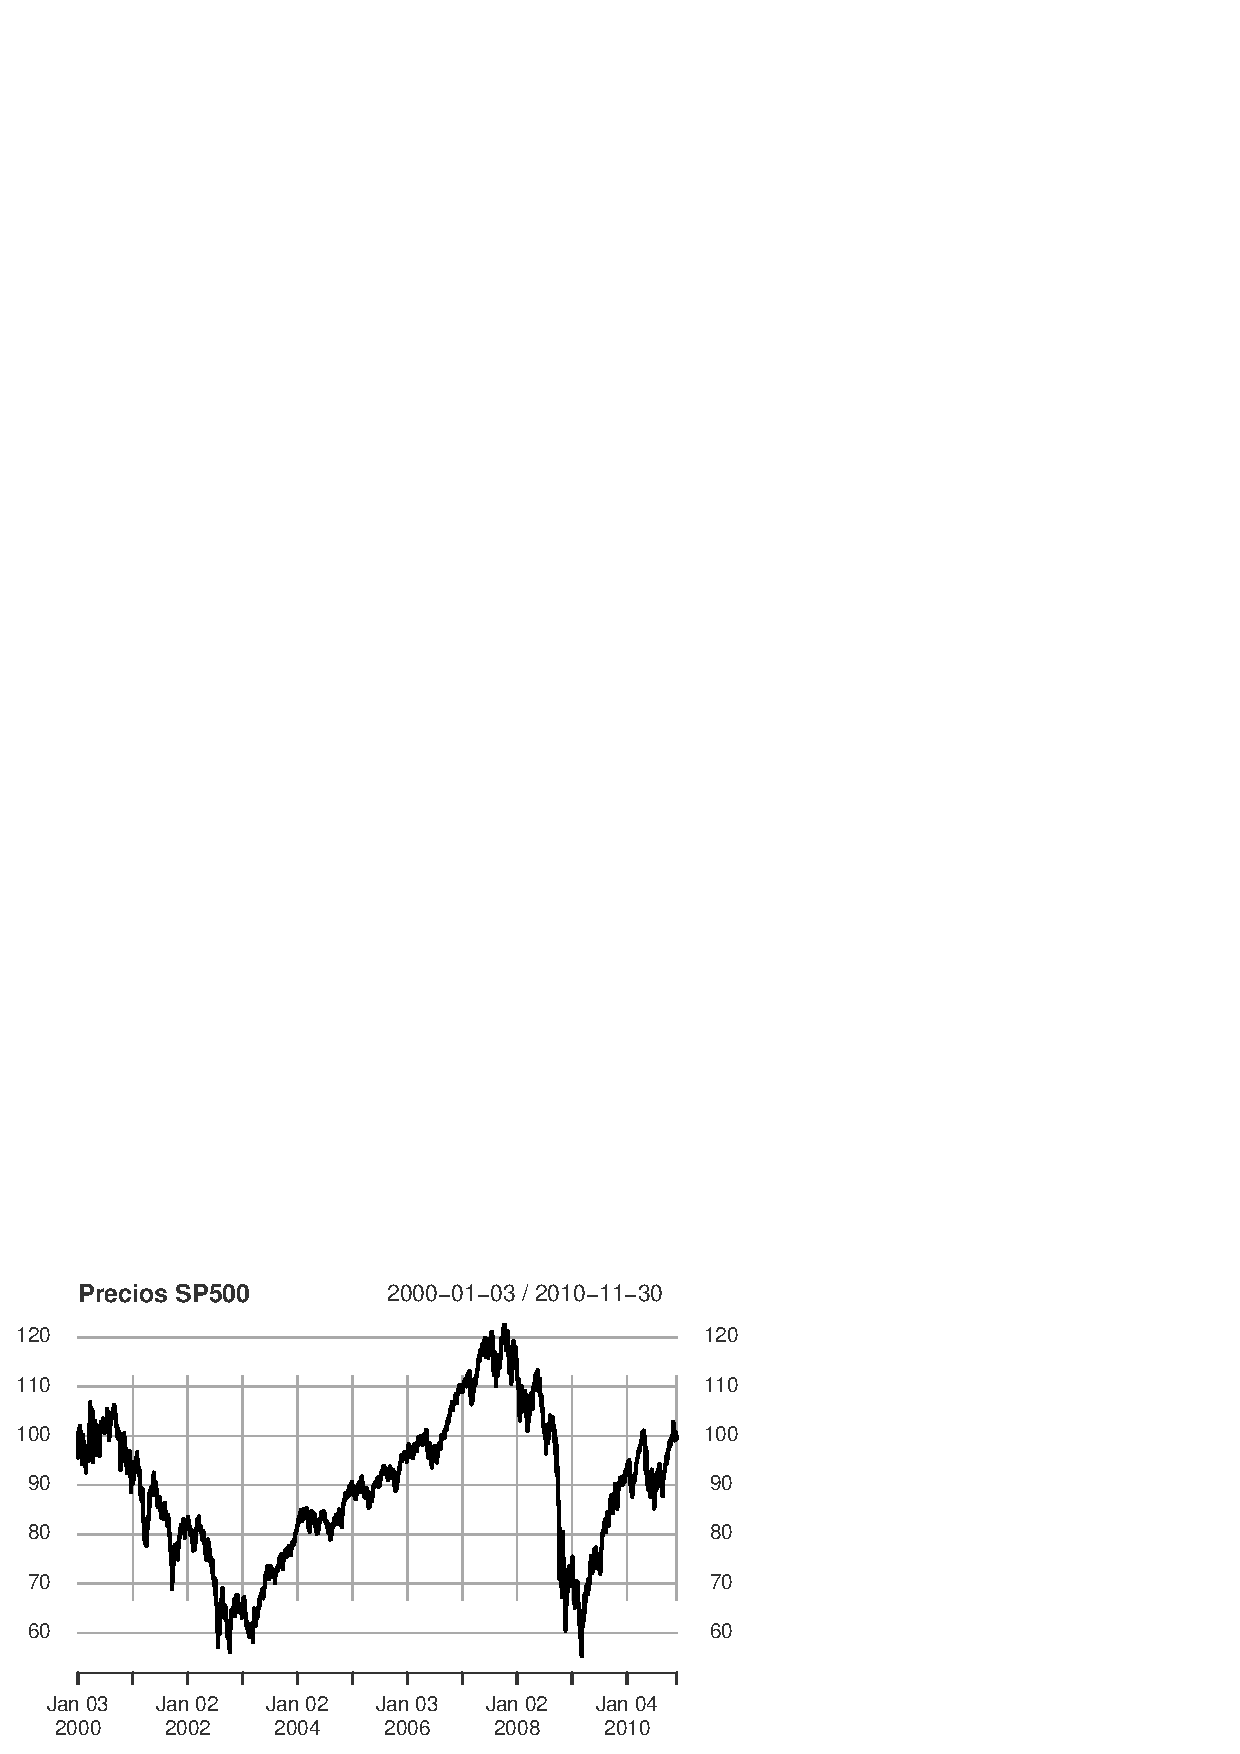
\includegraphics[scale=0.25]{spy.pdf}
\end{figure}

\end{frame}

%---------------------------------------------------------
%---------------------Slide 6--------------------------
\begin{frame}
\frametitle{Una excursi\'on al mundo no-lineal}
\textbf{Ejemplo de una serie financiera}\\
\textbf{Retornos diarios S$\&$P 500 - Ene90-Dic99}

\begin{figure}[t!]
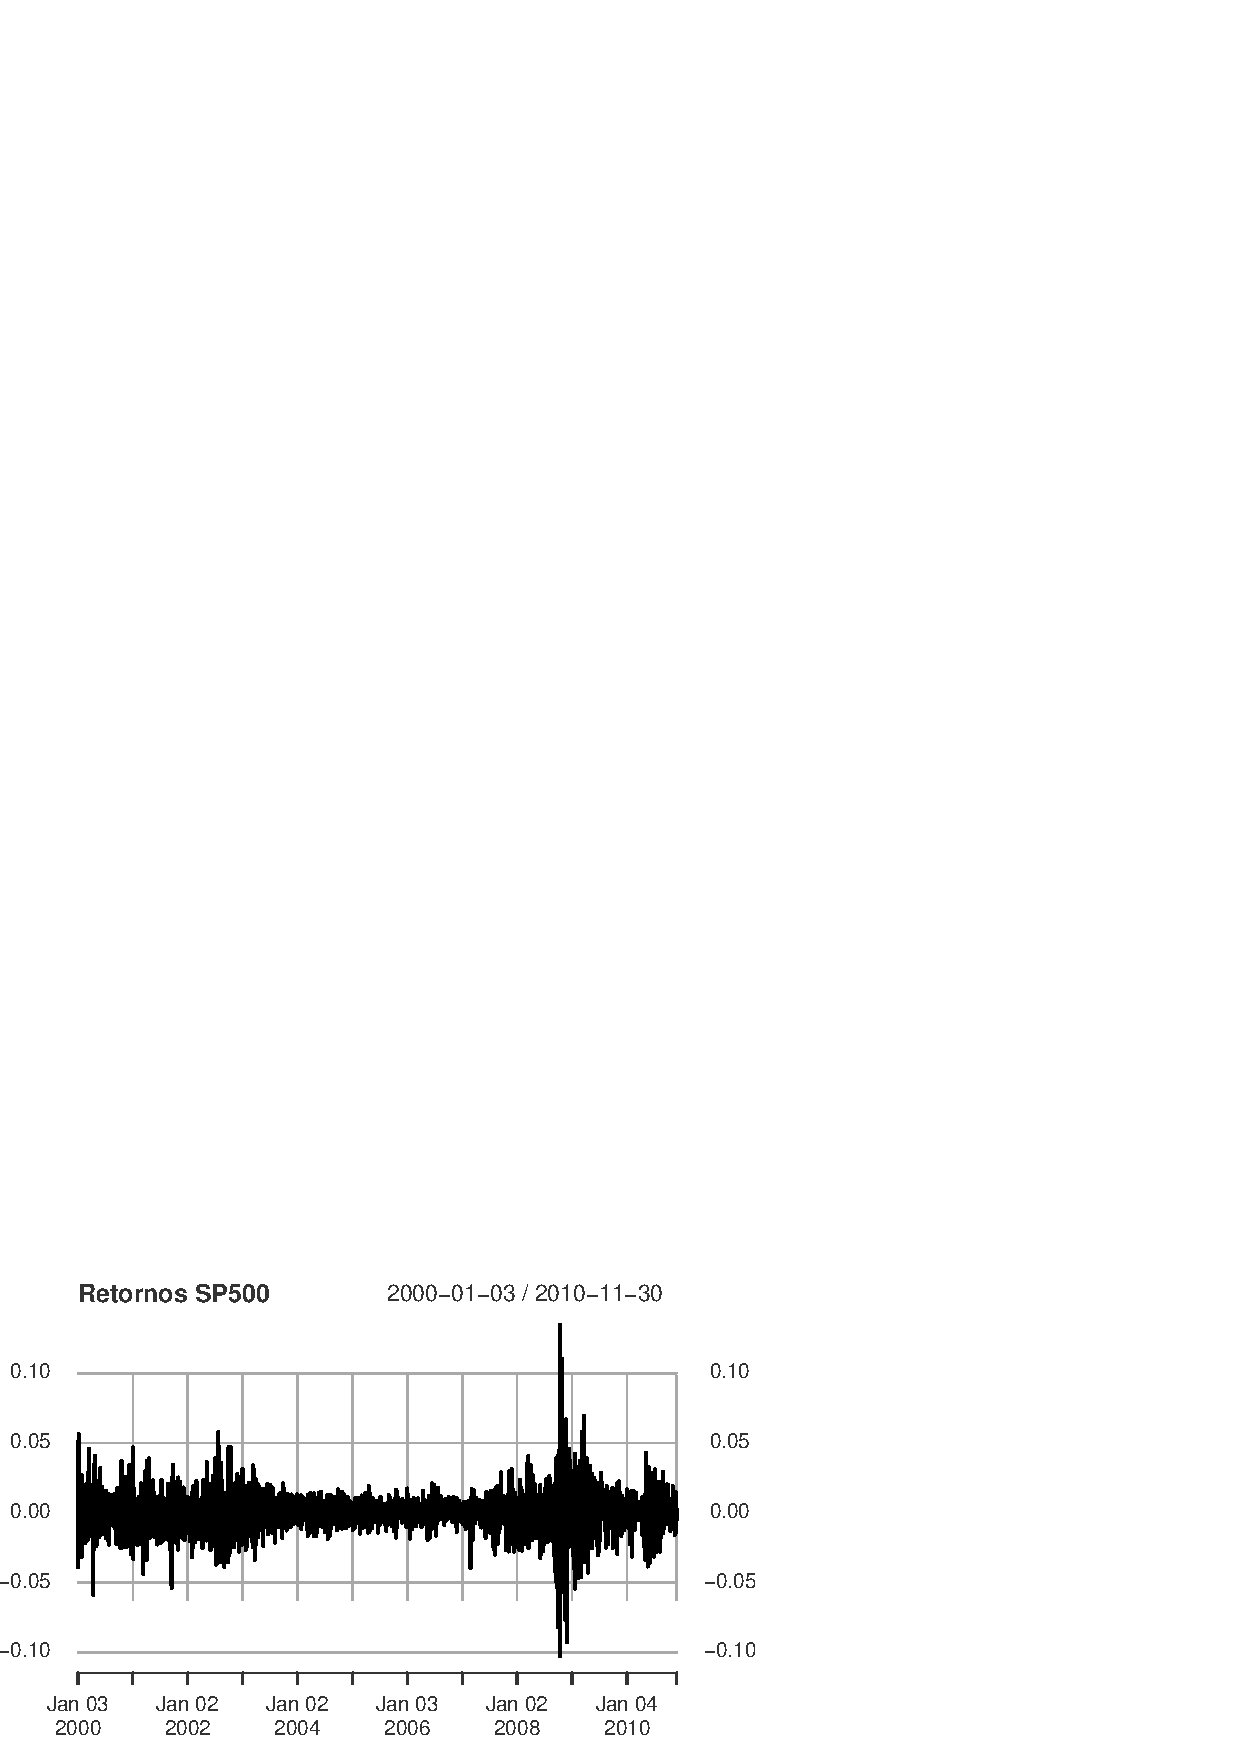
\includegraphics[scale=0.25]{Rspy.pdf}
\end{figure}

\end{frame}

%---------------------------------------------------------
%---------------------Slide 7--------------------------
\begin{frame}
\frametitle{Una excursi\'on al mundo no-lineal}

Nuestro modelo estructural ``tradicional" podr\'{i}a ser algo como:\\

\begin{equation}
Y_t = \beta_1 + \beta_2 X_{2t} + \beta_2 X_{2t} + \dots{} + \beta_k X_{kt} +\mu_t 
\end{equation}

donde $\mu_t$ = white noise, es decir $\mu_t \string~N(0,\sigma^2)$.\\
\vspace{4mm}	

\cite{campbell1997econometrics} definen un proceso de generaci\'on de datos no-lineal como uno que se puede escribir como:\\
\begin{equation}
Y_t = f(\mu_t,\mu_{t-1} ,\mu_{t-2},\dots{})
\end{equation}

donde $\mu_t$ es un t\'ermino de error aleatorio (iid) y $f$ es una funci\'on no lineal.\\
\vspace{4mm}	

\end{frame}

%---------------------------------------------------------
%---------------------Slide 8--------------------------
\begin{frame}
\frametitle{Una excursi\'on al mundo no-lineal}

Tambi\'en dan una definici\'on un poco m\'as espec\'{i}fica:
\begin{equation}
Y_t = g(\mu_{t-1} ,\mu_{t-2},\dots{}) + \mu_t \sigma^2(\mu_{t-1} ,\mu_{t-2},\dots{})
\end{equation}
donde g es una funci\'on de t\'erminos de error pasados solamente y  $\sigma^2$ es un t\'ermino de varianza.
\vspace{4mm}	

Modelos con $g(\cdot)$ no lineales, son ``no-lineales en la media", mientras que los no lineales en $\sigma^2(\cdot)$ son ``no-lineales en varianza".

\end{frame}

%---------------------------------------------------------
%---------------------Slide 9--------------------------
\begin{frame}
\frametitle{Tipos de modelos no lineales}

El paradigma lineal es muy \'util. Muchas relaciones aparentemente no lineales se pueden linealizar, a trav\'es de una transformaci\'on adecuada. Por otra parte, es probable que muchas relaciones en finanzas sean intr\'{i}nsecamente no lineales.\\
\vspace{4mm}	

Hay muchos tipos de modelos no lineales, e.g.\\
\only<1->{
\begin{itemize}
\item[-] ARCH / GARCH
\item[-] switching models
\item[-] bilinear models
\item[-] Redes neuronales
\end{itemize}
}
\end{frame}

%---------------------------------------------------------
%---------------------Slide 10--------------------------
\begin{frame}
\frametitle{Pruebas de no linealidad}

Las herramientas ``tradicionales" de an\'alisis de series temporales (ACF, an\'alisis espectral, etc.) pueden no encontrar evidencia de que podamos utilizar un modelo lineal, pero los datos a\'un pueden no ser independientes.\\
Se han desarrollado Pruebas de Portmanteau para la dependencia no-lineal. La m\'as simple es el RESET de Ramsey, que toma la forma: 	

\begin{equation}
\hat{\mu_t} = \beta_0 + \beta_1 \hat{y}^2+ \beta_2 \hat{y}^3+\dots{}\beta_{p-1} \hat{y}^p+ \nu_t
\end{equation}

Se dispone de muchas otras pruebas de no linealidad, por ejemplo, el ``test BDS" y la prueba de biespectro.\\
Un modelo no-lineal en particular que ha demostrado ser muy \'util en finanzas es el modelo ARCH, desarrollado por \cite{engle1982autoregressive}.

\end{frame}

%---------------------------------------------------------
%---------------------Slide 11--------------------------
\begin{frame}
\frametitle{Heteroscedasticidad Revisada}

Como vimos anteriormente, un ejemplo de un modelo estructural es:\\
\begin{equation}
Y_t = \beta_1 + \beta_2 X_{2t} + \beta_2 X_{2t} + \dots{} + \beta_k X_{kt} +\mu_t 
\end{equation}
\vspace{2mm}	

donde $\mu_t$ = white noise, es decir $\mu_t \string~N(0,\sigma^2)$.\\
\vspace{2mm}	

La suposici\'on de que la varianza de los errores es constante se conoce como homocedasticidad, i.e. $Var(\mu_t)=\sigma^2$\\
 \vspace{2mm}	

?`Qu\'e pasa si la varianza de los errores no es constante?\\

\textbf{heterocedasticidad}\\
\vspace{4mm}	

Lo que implican que las estimaciones de error est\'andar podr\'{i}an estar equivocadas.\\
En la pr\'actica  la varianza de los errores NO esconstante en el tiempo, por ejemplo para los datos financieros.

\end{frame}

%---------------------------------------------------------
%---------------------Slide 12--------------------------
\begin{frame}
\frametitle{Autoregressive Conditionally Heteroscedastic Models - Modelos ARCH }

Utilicemos un modelo que no asume que la varianza es constante.\\

Recuerde la definici\'on de la varianza de $\mu_t$:\\

\begin{equation}
\sigma_t^2 = Var(\mu_t | \mu_{t-1},  \mu_{t-2}, \dots{}) = E((\mu_t -E(\mu_{t}))^2 | \mu_{t-1},  \mu_{t-2}, \dots{})
\end{equation}
 \vspace{4mm}	


Normalmente suponemos que $E(\mu_t) = 0$, de aqu\'{i}:
\begin{equation}
\sigma_t^2 = Var(\mu_t | \mu_{t-1},  \mu_{t-2}, \dots{}) = E(\mu_{t}^2 | \mu_{t-1},  \mu_{t-2}, \dots{})
\end{equation} 

?`De qu\'e depender\'a el valor actual de la varianza de los errores?\\

\textbf{Del cuadrado de los t\'erminos de error anteriores}.\\

\end{frame}

%---------------------------------------------------------
%---------------------Slide 13--------------------------
\begin{frame}
\frametitle{Autoregressive Conditionally Heteroscedastic Models - Modelos ARCH }

Esto nos lleva al modelo conocido como ARCH, ``autoregressive conditionally heteroscedastic model" (modelo condicionalmente heterocedástico autorregresivo):

\begin{equation}
\sigma_t^2 = \alpha_0 + \alpha_1 \mu^2_{t-1}
\end{equation} 

En particular el modelo anterior representa un ARCH(1) model.


\end{frame}

%---------------------------------------------------------
%---------------------Slide 14--------------------------
\begin{frame}
\frametitle{Autoregressive Conditionally Heteroscedastic Models - Modelos ARCH }

El modelo completo es:

\begin{equation}
Y_t = \beta_1 + \beta_2 X_{2t} + \beta_2 X_{2t} + \dots{} + \beta_k X_{kt} +\mu_t, \mu_t \string~N(0,\sigma^2)
\end{equation}
\vspace{2mm}	
donde $\sigma_t^2 = \alpha_0 + \alpha_1 \mu^2_{t-1}$
\vspace{2mm}	
Podemos extender f\'acilmente esto para el caso general en que la varianza del error depende de $q$ rezagos de errores al cuadrado:
\begin{equation}
\sigma_t^2 = \alpha_0 + \alpha_1 \mu^2_{t-1} + \alpha_2 \mu^2_{t-2} + \dots{} + + \alpha_q \mu^2_{t-q}
\end{equation} 

Este es un modelo ARCH(q).

\end{frame}

%---------------------------------------------------------
%---------------------Slide 15--------------------------
\begin{frame}
\frametitle{Autoregressive Conditionally Heteroscedastic Models - Modelos ARCH }

En lugar de llamar a la varianza, $\sigma^2_t$ en la literatura se le suele llamar $h_t$, por lo que el modelo es en definitiva:

\begin{equation}
Y_t = \beta_1 + \beta_2 X_{2t} + \beta_2 X_{2t} + \dots{} + \beta_k X_{kt} +\mu_t, \mu_t \string~N(0,h)
\end{equation}
\vspace{2mm}	
donde 

\begin{equation}
h_t = \alpha_0 + \alpha_1 \mu^2_{t-1} + \alpha_2 \mu^2_{t-2} + \dots{} + + \alpha_q \mu^2_{t-q}
\end{equation} 

\end{frame}

%---------------------------------------------------------
%---------------------Slide 16--------------------------
\begin{frame}
\frametitle{Otra forma de representar a los ARCH Models}

Por ejemplo, considere un ARCH (1). En lugar de la representaci\'n anterior, podemos escribir 

\begin{equation}
Y_t = \beta_1 + \beta_2 X_{2t} + \beta_2 X_{2t} + \dots{} + \beta_k X_{kt} +\mu_t, \mu_t =\nu_t \sigma_t
\end{equation}
\vspace{2mm}	
donde 

\begin{equation}
\sigma_t = \sqrt{\alpha_0 + \alpha_1 \mu^2_{t-1}}
\end{equation} 

Las dos formas representas diferentes maneras de expresar exactamente el mismo modelo. La primera forma es m\'as f\'acil de entender, mientras que la segunda representa mejor la simulaci\'on de un modelo ARCH.

\end{frame}

%---------------------------------------------------------
%---------------------Slide 17--------------------------
\begin{frame}
\frametitle{La prueba del ``efecto ARCH"}

1.- En primer lugar, se corre una regresi\'on lineal, por ejemplo:

\begin{equation}
Y_t = \beta_1 + \beta_2 X_{2t} + \beta_2 X_{2t} + \dots{} + \beta_k X_{kt} +\mu_t
\end{equation}
y se guardan los residuos,

2. A continuaci\'n, los residuos se elevan al cuadrado, y se corre una regresi\'on sobre los $q$ rezagos propios para la prueba de ARCH de orden $q$, es decir, ejecutar la regresión
\begin{equation}
\hat{\mu_t^2} = \gamma_0 + \gamma_1 \hat{\mu_{t-1}}^2+ \gamma_2 \hat{\mu_{t-2}}^2+\dots{} +\gamma_{q} \hat{\mu_{t-q}}^2+ \nu_t
\end{equation}

3. El test estad\'{i}stico se define como TR2 (el n\'umero de observaciones multiplicado por el coeficiente de correlaci\'on m\'ultiple) a partir de la \'ultima regresi\'on, y se distribuye como una  $\chi^2(q)$.

\end{frame}

%---------------------------------------------------------
%---------------------Slide 18--------------------------
\begin{frame}
\frametitle{La prueba del ``efecto ARCH"}

4. Las hip\'otesis nula y alternativa son:
\vspace{2mm}	

	$H0 : \gamma_1 = 0 y \gamma_2 = 0 y \gamma_3 = 0 y \dots{} \gamma_q = 0.$
	\vspace{2mm}	

	$H1 : \gamma_1 \ne 0 y \gamma_2 \ne 0 y \gamma_3 \ne 0 y \dots{} \gamma_q \ne 0.$
\vspace{2mm}	
    
Si el valor de la prueba estad\'{i}stica es mayor que el valor cr\'{i}tico de la distribuci\'on $\chi^2(q)$, se rechaza la hip\'otesis nula.\\
\vspace{2mm}	

Tenga en cuenta que la prueba ARCH tambi\'en se aplica directamente a la rentabilidad, en lugar de a los residuos de la etapa 1 anterior.

\end{frame}

%---------------------------------------------------------
%---------------------Slide 19--------------------------
\begin{frame}
\frametitle{Principales problemas de los mdoelos ARCH}

?`C\'omo decidimos el mejor q?\\

El valor requerido de q podría ser muy grande\\

Las restricciones de no negatividad pueden ser violadas.\\

Cuando se estima un modelo ARCH, requerimos $\alpha_i >0$ $\forall i=1,2,...,q$ (ya que la varianza no puede ser negativa)

Una extensi\'n natural de un modelo ARCH (q), que evita algunos de estos problemas es el modelo GARCH que veremos a continuaci\'on.


\end{frame}
\end{section}

%---------------------------------------------------------
%---------------------Slide 20--------------------------
\begin{section}{Modelos GARCH}
\begin{frame}
\frametitle{Generalised ARCH - GARCH Models}

Introducido por \cite{bollerslev1986generalized} deja que la varianza condicional sea dependiente de sus propios rezagos. De esta forma, la ecuaci\'n de la varianza es ahora:

\begin{equation} \label{eqn:p}
\sigma_t^2 = \alpha_0 + \alpha_1 \mu^2_{t-1} + \beta \sigma_{t-1}^2
\end{equation} 
								
Se trata de un GARCH (1,1), que es equivalente a un ARMA (1,1) de la ecuaci\'on de la varianza.\\

También podríamos escribir

\begin{equation} \label{eqn:q}
\sigma_{t-1}^2 = \alpha_0 + \alpha_1 \mu^2_{t-2} + \beta \sigma_{t-2}^2
\end{equation} 

\begin{equation} \label{eqn:r}
\sigma_{t-2}^2 = \alpha_0 + \alpha_1 \mu^2_{t-3} + \beta \sigma_{t-3}^2
\end{equation} 

\end{frame}

%---------------------------------------------------------
%---------------------Slide 21--------------------------
\begin{frame}
\frametitle{Generalised ARCH - GARCH Models}

Sustituyendo \eqref{eqn:q} en \eqref{eqn:p}

\begin{equation} \label{eqn:p}
\sigma_t^2 = \alpha_0 + \alpha_1 \mu^2_{t-1} + \beta (\alpha_0 + \alpha_1 \mu^2_{t-2} + \beta \sigma_{t-2}^2)
\end{equation} 

\begin{equation} \label{eqn:p}
\sigma_t^2 = \alpha_0 (1 + \beta) + \alpha_1 \mu^2_{t-1} (1 + \beta L) + \beta \sigma_{t-1}^2
\end{equation} 

Si seguimos reemplazando t\'erminos,  el modelo GARCH(1,1)  puede escribirse como un modelo ARCH de orden infinito.
 
As\'{i}, podemos extender el GARCH (1,1) a un GARCH (p, q):
\begin{equation}
\sigma_{t}^{2}=\alpha_{0}+\sum_{i=1}^{q}\alpha_{i}\mu_{t-i}^{2}+\sum_{j=1}^{p}\beta_{j}\sigma_{t-j}^{2}
\end{equation}

\end{frame}

%---------------------------------------------------------
%---------------------Slide 22--------------------------
\begin{frame}
\frametitle{Generalised ARCH - GARCH Models}

En general, un modelo GARCH(1,1)  es suficiente para capturar la volatilidad clusterizada de los datos.\\
\begin{equation}
\sigma_{t}^{2}=\alpha_{0}+\alpha_{1}\mu_{t-1}^{2}+\beta_{1}\sigma_{t-1}^{2}
\end{equation}

\vspace{2mm}	

?`Por qu\'e es mejor un modelo GARCH que un modelo ARCH?\\
\vspace{2mm}	

- Es m\'as parsimonioso - evita el sobreajuste\\
- Menos probabilidades de violar restricciones de no negatividad


\end{frame}

%---------------------------------------------------------
%---------------------Slide 23--------------------------
\begin{frame}
\frametitle{La varianza incondicional bajo la especificación GARCH}

Calculando la varianza incondicional, podemos estimar la desviaci\'on est\'andar que estamos buscando. De esta forma, derivaremos la varianza incondicional a partir de los modelos ARCH y GARCH. Adem\'as, se presenta una nota sobre la variación diaria de escala.\\
\vspace{2mm}	

\textbf{ARCH Unconditional Variance}\\

Suponemos un proceso que podr\'{i}a representarse mediante un modelo econom\'etrico, por ejemplo:\\
\begin{equation}
y_{t}=\mu+\epsilon_{t}
\end{equation}


with $\epsilon_{t}\sim\left(0,\sigma_{t}^{2}\right)$

Asumimos que la varianza condicional sigue un modelo del tipo ARCH (1), es decir:\\
\begin{equation}
\sigma_{t}^{2}=\alpha_{0}+\alpha_{1}\epsilon_{t-1}^{2}
\end{equation}

\end{frame}

%---------------------------------------------------------
%---------------------Slide 24--------------------------
\begin{frame}
\frametitle{La varianza incondicional bajo la especificación GARCH}


Usando el operador de expectativa incondicional, tenemos:

\[
\mathbb{E}\left(\sigma_{t}^{2}\right)=\sigma_{t}^{2}
\]


\[
\mathbb{E}\left(\alpha_{0}\right)=\alpha_{0}
\]


\[
\mathbb{E}\left(\epsilon_{t-1}^{2}\right)=\sigma_{t}^{2}
\]


\medskip{}


Tenemos:\\
\begin{equation}
\sigma_{t}^{2}\left(1-\alpha_{1}\right)=\alpha_{0}
\end{equation}


\begin{equation}
\Rightarrow\sigma_{t}^{2}=\frac{\alpha_{0}}{1-\alpha_{1}}
\end{equation}


\medskip{}

\end{frame}

%---------------------------------------------------------
%---------------------Slide 25--------------------------
\begin{frame}
\frametitle{La varianza incondicional bajo la especificación GARCH}


Si generalizamos a un modelo ARCH (q), obtenemos:\\
\begin{eqnarray}
\sigma_{t}^{2} & = & \alpha_{0}+\alpha_{1}\epsilon_{t-1}^{2}+\alpha_{2}\epsilon_{t-2}^{2}+\cdots+\alpha_{q}\epsilon_{t-q}^{2}\nonumber \\
 & = & \alpha_{0}+\sum_{k=1}^{q}\alpha_{k}\epsilon_{t-k}^{2}
\end{eqnarray}


donde:

\[
\mathbb{E}\left(\epsilon_{t-1}^{2}\right)=\mathbb{E}\left(\epsilon_{t-2}^{2}\right)=\cdots=\mathbb{E}\left(\epsilon_{t-q}^{2}\right)=\sigma_{t}^{2}
\]


entonces:

\begin{eqnarray}
\sigma_{t}^{2} & = & \frac{\alpha_{0}}{1-\alpha_{1}-\alpha_{2}-\cdots-\alpha_{q}}\nonumber \\
 & = & \cfrac{\alpha_{0}}{1-\sum_{k=1}^{q}\alpha_{k}}
\end{eqnarray}


\end{frame}

%---------------------------------------------------------
%---------------------Slide 26--------------------------
\begin{frame}
\frametitle{La varianza incondicional bajo la especificación GARCH}

\textbf{GARCH Unconditional Variance}\\

Supongamos el mismo proceso dado previamente, pero esta vez la varianza
tambi\'en depende de sus propios $p$ lags:

\begin{eqnarray}
\sigma_{t}^{2} & = & \alpha_{0}+\alpha_{1}\epsilon_{t-1}^{2}+\alpha_{2}\epsilon_{t-2}^{2}+\cdots+\alpha_{q}\epsilon_{t-q}^{2}+\beta_{1}\sigma_{t-1}^{2}+\beta_{2}\sigma_{t-2}^{2}+\cdots+\beta_{p}\sigma_{t-p}^{2}\nonumber \\
 & = & \alpha_{0}+\sum_{k=1}^{q}\alpha_{k}\epsilon_{t-k}^{2}+\sum_{l=1}^{p}\alpha_{l}\sigma_{t-l}^{2}
\end{eqnarray}


La ecuación anterior da un modelo GARCH (p, q). Utilizando\\

$\mathbb{E}\left(\sigma_{t-1}^{2}\right)=\mathbb{E}\left(\sigma_{t-2}^{2}\right)=\cdots=\mathbb{E}\left(\sigma_{t-p}^{2}\right)=\sigma_{t}^{2}$\\


De esta forma tenemos: 

\begin{eqnarray}
\sigma_{t}^{2} & = & \frac{\alpha_{0}}{1-\alpha_{1}-\alpha_{2}-\cdots-\alpha_{q}-\beta_{1}-\beta_{2}-\cdots-\beta_{p}}\nonumber \\
 & = & \cfrac{\alpha_{0}}{1-\sum_{k=1}^{q}\alpha_{k}-\sum_{l=1}^{p}\beta_{l}}
\end{eqnarray}
\\
\end{frame}

%---------------------------------------------------------
%---------------------Slide 27-------------------------
\begin{frame}
\frametitle{La varianza incondicional bajo la especificación GARCH}

\begin{itemize}
\item \textbf{Scaling Volatility}
\end{itemize}
El c\'alculo de la volatilidad y la escala en diferentes horizontes de tiempo es
posible solo en los casos en que los cambios en el registro del precio del activo $v_ {t}$ se distribuyen de forma independiente e idéntica (iid).

\begin{center}
\begin{equation}
v_{t}=v_{t-1}+\varepsilon_{t}\qquad\varepsilon_{t}\sim(0,\sigma^{2})
\end{equation}
$ $
\par\end{center}

Entonces 1-day return es: 

\begin{center}
\[
v_{t}-v_{t-1}=\varepsilon_{t}
\]

\par\end{center}

con desviaci\'on est\'andar $\sigma$. 
\end{frame}

%---------------------------------------------------------
%---------------------Slide 28--------------------------
\begin{frame}
\frametitle{La varianza incondicional bajo la especificación GARCH}

Similarmente, el h-day return es: 

\begin{center}
\begin{equation}
v_{t}-v_{t-h}=\sum_{i=0}^{h-1}\varepsilon_{t-i}
\end{equation}

\par\end{center}

con varianza $h\sigma^{2}$ y desviaci\'on est\'andar $\sqrt{h\sigma^{2}}$.
\\
Sin embargo, los rendimientos de los activos financieros de alta frecuencia claramente no son iid ... pero sigue siendo una buena aproximaci\'on.

\end{frame}
\end{section}

%---------------------------------------------------------
%---------------------Slide 29--------------------------

\begin{section}{Estimaci\'on de modelos ARCH / GARCH}
\begin{frame}
\frametitle{Estimaci\'on de modelos ARCH / GARCH}

Dado que el modelo ya no es de la forma lineal que acostumbramos, no podemos usar MCO.\\
\\
Utilizamos otra t\'ecnica conocida como de m\'axima verosimilitud.\\
\\
El m\'etodo funciona mediante la b\'usqueda de los valores m\'as probables de los par\'ametros, dados los datos reales.\\
\\
M\'as específicamente, construimos una funci\'on de verosimilitud y la maximizamos. 


\end{frame}

%---------------------------------------------------------
%---------------------Slide 30--------------------------
\begin{frame}
\frametitle{Estimaci\'on de modelos ARCH / GARCH}

Los pasos a seguir en la estimaci\'n de un modelo ARCH o GARCH son los siguientes:\\
1.- Especificar las ecuaciones apropiadas para la media y la varianza - por ejemplo, un AR (1) - GARCH (1,1):\\

\begin{equation}
y_{t}=\alpha+\phi y_{t-1}+\mu_t, \mu_t \string~N(0,\sigma^2)
\end{equation}
\begin{equation}
\sigma_{t}^{2}=\alpha_{0}+\alpha_{1}\mu_{t-1}^{2}+\beta_{1}\sigma_{t-1}^{2}
\end{equation}

2.- Especifique la función de verosimilitud para maximizar:\\

\begin{equation}
L = - (T/2)log(2 \pi) - (1/2) \sum_{t=1}^{T} log(\sigma_{t}^{2}) - (1/2) \sum_{t=1}^{T} (y_t - \alpha-\phi y_{t-1})/\sigma_{t}^{2}
\end{equation}

3. El computador maximizar la funci\'on, y calcula los par\'ametros y sus errores est\'andares…\\


\end{frame}
\end{section}

%---------------------------------------------------------
%---------------------Slide 31--------------------------
\begin{section}{Extensiones al modelo GARCH b\'asico}
\begin{frame}
\frametitle{Extensiones al modelo GARCH b\'asico}

Los principales problemas de los modelos GARCH (p, q) son:\\
- Restricciones de no negatividad pueden ser violadas\\
- Los Modelos GARCH no pueden dar cuenta de los efectos de apalancamiento\\
\vspace{2mm}	

En este contexto, desde que se desarroll\'o el modelo GARCH, se han propuesto un gran n\'umero de extensiones y variantes. Tres de los ejemplos m\'as importantes son los modelos GARCH-M, EGARCH, y GJR. \\
\vspace{2mm}	

De hecho, posibles soluciones a los dos problemas planteados anteriormente, pueden ser abordados por el modelo GARCH exponencial (EGARCH) o el modelo GJR, que plantean modelos GARCH asim\'etricos. 

\end{frame}

%---------------------------------------------------------
%---------------------Slide 32--------------------------
\begin{frame}
\frametitle{GARCH - in Mean}

Basados en el problema cl\'asico de cobertura de riesgo, si esperamos que un riesgo se compense con una mayor rentabilidad, ?`por qu\'e no dejar que el retorno de un valor determinado sea parcialmente determinado por su riesgo?
\vspace{2mm}	

\cite{engle1987estimating} sugirieron la especificaci\'on ARCH-M:

\begin{equation}
Y_t = \mu + \delta \sigma_{t-1} + \mu_t , \mu_t \string~N(0,\sigma^2_t)
\end{equation}

\begin{equation}
\sigma^2_t = \alpha_0 + \alpha_1 \mu^2_{t-1} + \beta \mu^2_{t-1}
\end{equation} 

$\delta$ puede interpretarse como una especie de prima por riesgo.

Es posible combinar todos o algunos de estos modelos en conjunto para obtener modelos m\'as complejos, h\'{i}bridos - por ejemplo, un modelo del tipo ARMA-EGARCH (1,1)-M.

\end{frame}

%---------------------------------------------------------
%---------------------Slide 32--------------------------
\begin{frame}
\frametitle{Modelo EGARCH}

Sugerido por \cite{nelson1991conditional} La ecuaci\'on de varianza est\'a dada por: 

\begin{equation}
\log(\sigma^2_t) = \omega + \beta log(\sigma^2_{t-1}) + \gamma \frac{\mu_{t-1}}{\sqrt{\sigma^2_{t-1}}} + \alpha \left[ \frac{|\mu_{t-1}|}{\sqrt{\sigma^2_{t-1}}} - \sqrt{\frac{2}{\pi}} \right]
\end{equation} 
\vspace{2mm}	

Ventajas del modelo\\
Dado que modelamos $log(\sigma^2_t)$, incluso si los par\'ametros son negativos, $\sigma^2_t$ ser\'a positivo.
Podemos tomar cuenta el efecto de apalancamiento: si la relaci\'on entre volatilidad y rentabilidad es negativa, $\gamma$, ser\'a negativo.

\end{frame}
\end{section}

%---------------------------------------------------------
%---------------------Slide 34--------------------------
\begin{frame}
\frametitle{Modelo GJR}

Debido a \cite{glosten1993relation}:

\begin{equation}
\sigma^2_t = \alpha_0 + \alpha_1 \mu^2_{t-1} + \beta \sigma^2_{t-1} + \gamma \mu^2_{t-1} I_{t-1}
\end{equation} 
\vspace{2mm}	

Donde:\\ 
$I_{t-1}=1$ si $\mu_{t-1} < 0$\\
$I_{t-1}=0$ si $\mu_{t-1} \geq 0$\\
\vspace{2mm}	

Para un efecto de apalancamiento ver\'{i}amos $\gamma > 0$.\\
\vspace{2mm}	

Requerimos $\alpha_1 + \gamma \geq 0$ y $\alpha_1 \geq 0$ para no-negatividad. 

\end{frame}
%---------------------------------------------------------
%---------------------Slide 35--------------------------
\begin{frame}
\frametitle{Modelos GARCH Multivariados}

Los modelos GARCH multivariados se utilizan para estimar y pronosticar covarianzas y correlaciones. La formulaci\'on b\'asica es similar a la del modelo GARCH, pero cuando a las varianzas, as\'{i} como tambi\'en a las covarianzas, se les permita variar en el tiempo.\\
\vspace{2mm}	

Hay 3 clases principales de formulaci\'on GARCH multivariante, que son ampliamente utilizadas: VECH, diagonal VECH y BEKK.\\
\vspace{2mm}	

Los modelos GARCH multivariantes (MGARCH) generalizan los modelos GARCH univariantes y permiten incorporar relaciones entre los procesos de volatilidad de varias series. Queremos saber por ejemplo,  c\'omo los cambios en la volatilidad de una acci\'on afectan a la volatilidad de otra acci\'on. Estas relaciones se pueden parametrizar de varias maneras. 

\end{frame}
\end{section}

%---------------------------------------------------------
%---------------------Slide 36--------------------------
\begin{frame}
\frametitle{GARCH vs volatilidad promedio retorno}

\only<1|handout:1>{
\begin{exampleblock}{C\'odigo en R}

getSymbols(``ECH", from=``2008-01-01")\\
Returns = diff(log(Ad(ECH)))\\
adf.test(Ad(ECH))\\
adf.test(Returns)\\
Returns[as.character(head(index(Ad(ECH)),1))] = 0\\
fit.garch $<-$ garch(Returns, trace=FALSE)\\
print(fit.garch)\\
coeftest(fit.garch)\\
sigmaGarch$<-$fit.garch[[``coef"]][[``a0"]]/(1-fit.garch[[``coef"]][[``a1"]]-fit.garch[[``coef"]][[``b1"]])\\
sigmaAvg$<-$var(Returns)\\

\end{exampleblock}
}

\end{frame}

%---------------------------------------------------------
%---------------------Slide 37--------------------------
\begin{frame}
\frametitle{GARCH vs volatilidad promedio retorno}

\begin{figure}[t!]
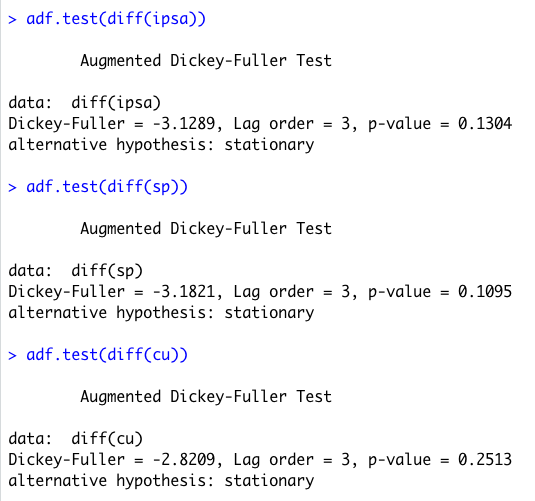
\includegraphics[scale=0.5]{adf.png}
\end{figure}

\end{frame}

%---------------------------------------------------------
%---------------------Slide 38--------------------------
\begin{frame}
\frametitle{GARCH vs volatilidad promedio retorno}

\begin{figure}[t!]
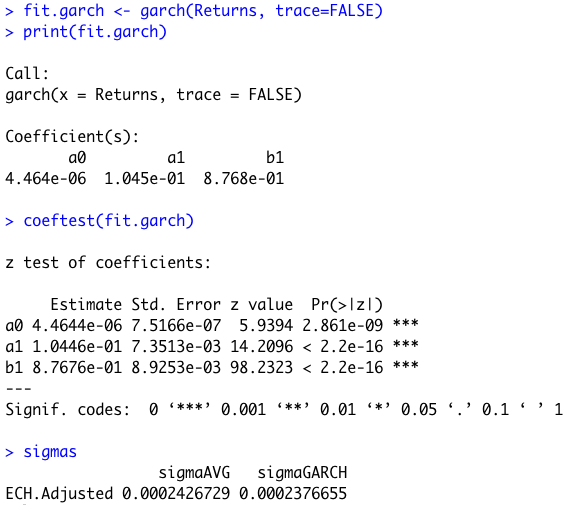
\includegraphics[scale=0.45]{garch.png}
\end{figure}

sigmaAvg     = 0.0002529142\\
sigmaGarch = 0.0002637039\\

\end{frame}

%---------------------------------------------------------
%---------------------Slide 39--------------------------
\begin{frame}
\frametitle{GARCH vs volatilidad promedio retorno}

\only<1|handout:1>{
\begin{exampleblock}{C\'odigo en R}

windowLength = 40\\
foreLength = length(Returns) - windowLength\\
sigmaAvgV $<-$ vector(mode=``character", length=foreLength)\\
sigmaGarchV $<-$ vector(mode=``character", length=foreLength)\\

\end{exampleblock}
}

\end{frame}

%---------------------------------------------------------
%---------------------Slide 39--------------------------
\begin{frame}
\frametitle{GARCH vs volatilidad promedio retorno}

\only<1|handout:1>{
\begin{exampleblock}{C\'odigo en R}
{\small
for (d in 1:foreLength) $\big\{$\\
$&&$ ReturnsOffset = Returns[(d):(windowLength+d)] \\
$&&$ fit.garch $<-$ garch(ReturnsOffset, trace=FALSE)\\
$&&$ sigmaGarch$<-$fit.garch[[``coef"]][[``a0"]]/(1-fit.garch[[``coef"]][[``a1"]]-fit.garch[[``coef"]][[``b1"]])\\
$&&$ sigmaAvg$<-$var(ReturnsOffset)\\
$&&$ print(sigmaGarch);print(sigmaAvg)\\
$&&$ sigmaGarchV[d]$<-$sigmaGarch\\
$&&$ sigmaAvgV[d]$<-$sigmaAvg\\
$\big\}$\\

plot.ts(sigmaAvgV, col = ``red", main=``Volatility Average versus GARCH(1,1)")\\
lines.default(sigmaGarchV, col = ``black")\\
}
\end{exampleblock}
}

\end{frame}

%---------------------------------------------------------
%---------------------Slide 41--------------------------
\begin{frame}
\frametitle{GARCH vs volatilidad promedio retorno}
\textbf{Retornos diarios ECH - 1Ene2008-today}

\begin{figure}[t!]
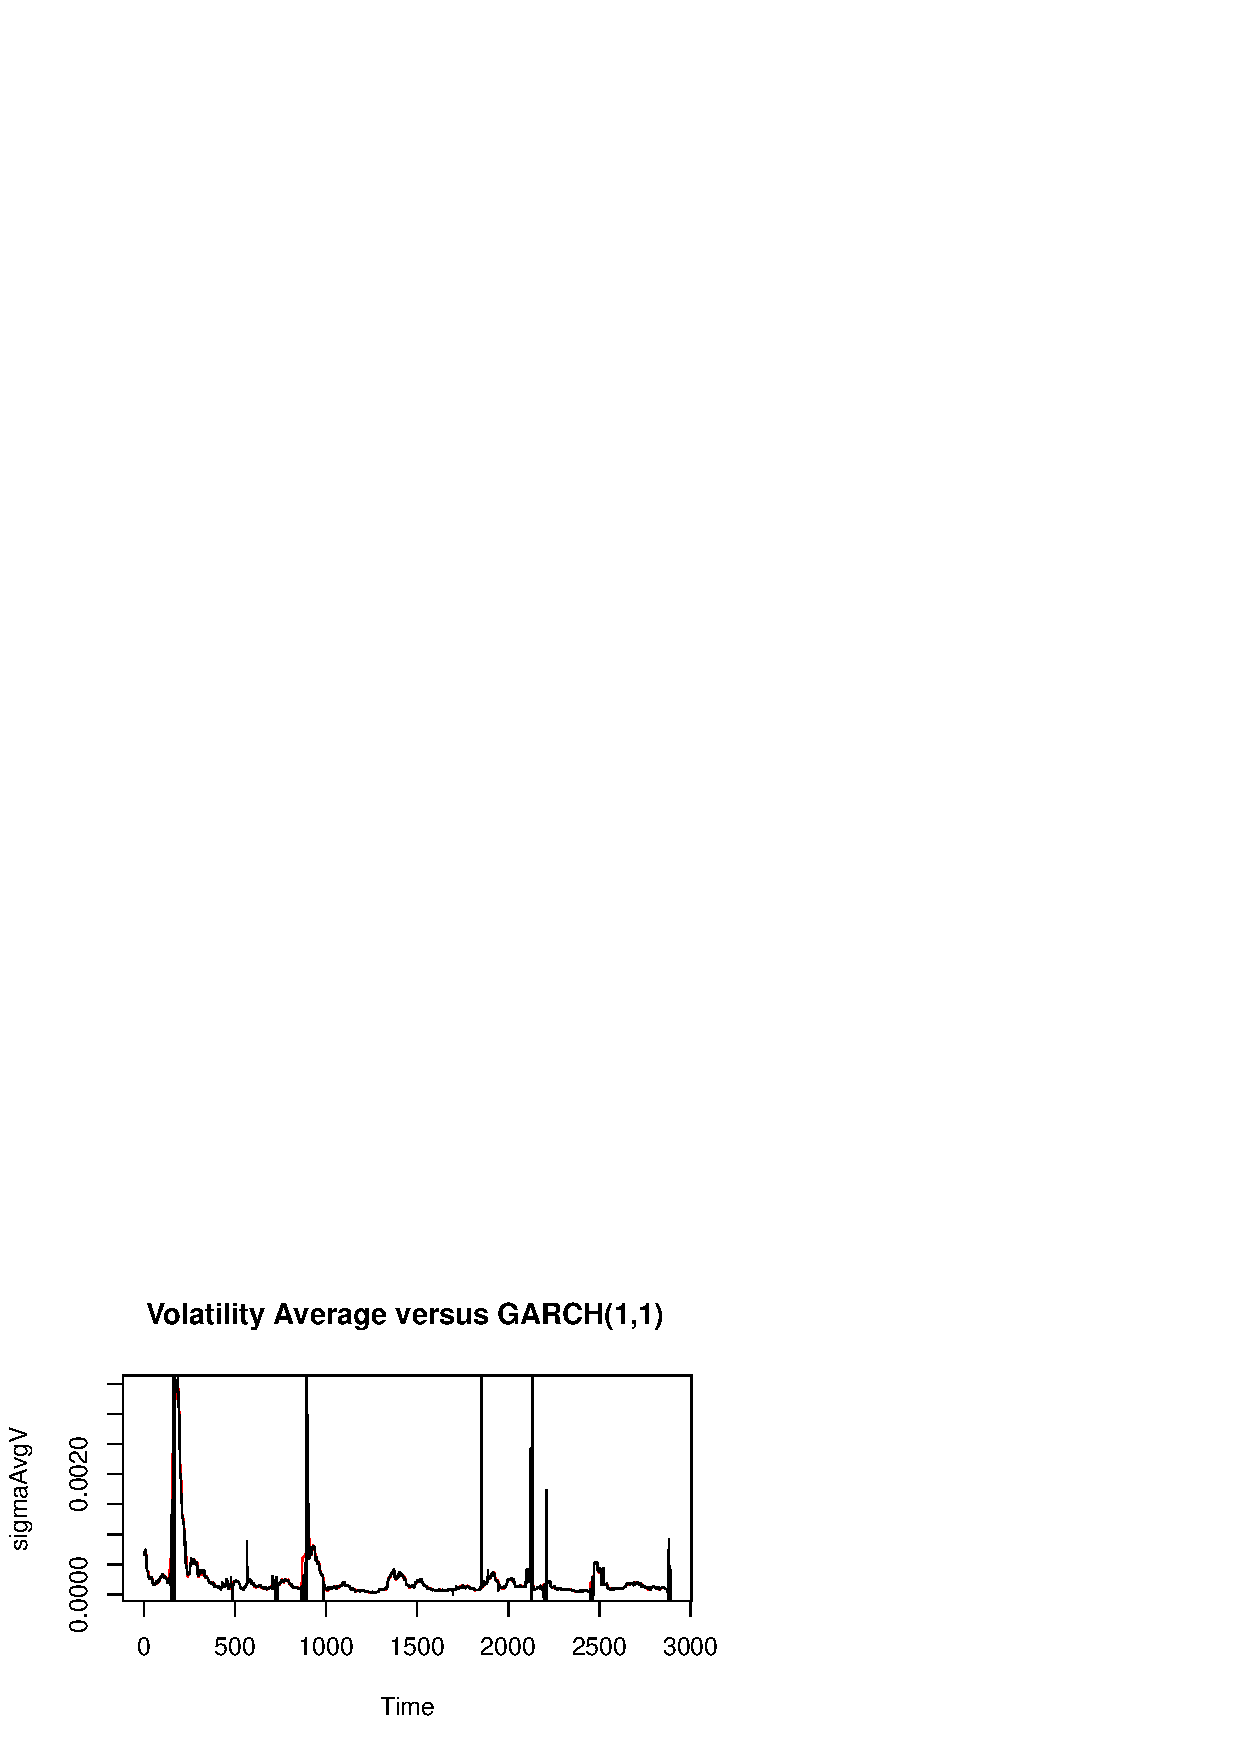
\includegraphics[scale=0.3]{volECH.png}
\end{figure}

\end{frame}

%---------------------------------------------------------
%---------------------Slide 42--------------------------
\begin{frame}
\frametitle{GARCH vs volatilidad promedio retorno}
\textbf{https://vlab.stern.nyu.edu/analysis/VOL.ECH:US-R.GARCH}

\begin{figure}[t!]
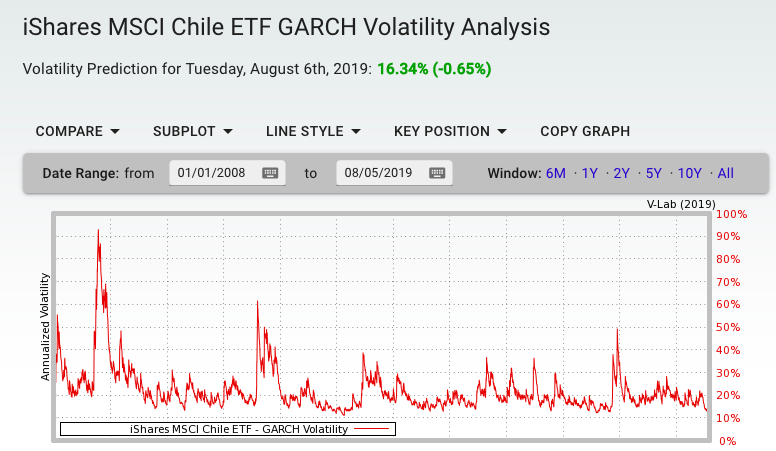
\includegraphics[scale=0.3]{v-lab.png}
\end{figure}

\end{frame}

%---------------------------------------------------------
%--------------Slide Referencias---------------------

\begin{section}{Referencias}
\begin{frame}[allowframebreaks]
        \frametitle{Referencias}
        \bibliographystyle{unsrt}
%        \nocite{*} %lista sin citar.
        \bibliography{TS_ref}
\end{frame}
\end{section}

%---------------------------------------------------------
\end{document} 
%---------------------------------------------------------




